\documentclass[11pt]{article}

\usepackage[a4paper,margin=1in]{geometry}
\usepackage{fontspec}
\usepackage{amsmath,amssymb}
\usepackage{graphicx}
\usepackage{xcolor}
\usepackage{microtype}
\emergencystretch=2.5em
\sloppy

% Palette from harchaoui.org/warith/colors/, reused for every TikZ diagram
% and for section headings, so the printed document and the diagrams read
% as one visual system rather than two unrelated styles.
\definecolor{CBlue}{HTML}{007AFF}
\definecolor{CBlueLight}{HTML}{CCE4FF}
\definecolor{CGreen}{HTML}{28CD41}
\definecolor{CGreenLight}{HTML}{D4F5D9}
\definecolor{CPurple}{HTML}{AF52DE}
\definecolor{CPurpleLight}{HTML}{EFDCF8}
\definecolor{COrange}{HTML}{FF9500}
\definecolor{COrangeLight}{HTML}{FFEACC}
\definecolor{CText}{HTML}{2B2926}

\usepackage{tikz}
\usetikzlibrary{arrows.meta,positioning}

\usepackage[style=authoryear,backend=biber]{biblatex}
\addbibresource{references.bib}

\usepackage{booktabs}
\usepackage{caption}
\usepackage{enumitem}
\usepackage{parskip}
\graphicspath{{img/}}

\usepackage{titlesec}
\titleformat{\section}{\normalfont\Large\bfseries\color{CBlue}}{\thesection}{0.6em}{}
\titleformat{\subsection}{\normalfont\large\bfseries\color{CBlue}}{\thesubsection}{0.6em}{}

\usepackage[colorlinks=true,linkcolor=CBlue,citecolor=CBlue,urlcolor=CBlue]{hyperref}

% Shared TikZ node styles for every diagram in this document: rounded
% rectangles, one fill/stroke pair per role (input, transform, technique,
% output), matching the palette above exactly.
\tikzstyle{ioNode}=[rectangle, rounded corners=6pt, draw=CBlue, fill=CBlueLight,
  thick, text width=3.1cm, align=center, minimum height=1.05cm, font=\small]
\tikzstyle{transformNode}=[rectangle, rounded corners=6pt, draw=CGreen, fill=CGreenLight,
  thick, text width=3.1cm, align=center, minimum height=1.05cm, font=\small]
\tikzstyle{techniqueNode}=[rectangle, rounded corners=6pt, draw=CPurple, fill=CPurpleLight,
  thick, text width=3.1cm, align=center, minimum height=1.05cm, font=\small]
\tikzstyle{outputNode}=[rectangle, rounded corners=6pt, draw=COrange, fill=COrangeLight,
  thick, text width=3.1cm, align=center, minimum height=1.05cm, font=\small]
\tikzstyle{arr}=[-{Latex[length=2.2mm]}, thick, draw=gray!65]

\title{\color{CBlue}Cartography Methodology}
\author{Warith Harchaoui}
\date{\today}

\begin{document}
\maketitle

This document is the technical record of how \texttt{sprezzature-maps} draws
a map: which projections, which color spaces, which terrain-shading
algorithm, which vendored datasets, and why each choice won out over the
available alternatives. It exists so a reader, including a future
maintainer of this repository, can reconstruct every rendering decision
from first principles rather than take on faith that a decision was made.

Two generators are covered: \texttt{choropleth} (\texttt{scripts/make\_choropleth.py}),
which fills each country on a world map by a per-country value, and
\texttt{situation\_map} (\texttt{scripts/make\_situation\_map.py}), which draws an
auto-centered regional plate. Both draw hand-authored images in a
resolution-independent vector format (Scalable Vector Graphics, SVG):
no charting library, no raster renderer, no \texttt{matplotlib}. Formulas
appear here in full so a reader does not have to open the source files'
own extensive docstrings to follow the reasoning; code references point
back to the exact function for a reader who wants the implementation, not
only the theory.

This source compiles with \texttt{xelatex} and \texttt{biber} to a fixed-layout
document (Portable Document Format, PDF):

\begin{verbatim}
cd doc
xelatex CARTOGRAPHY.tex
biber CARTOGRAPHY
xelatex CARTOGRAPHY.tex
xelatex CARTOGRAPHY.tex
\end{verbatim}

\tableofcontents

\section{Pipeline overview}

Both generators share a shape: project, color, shade relief, then compose
the result into one vector image. They differ in every specific: a
different projection, a different boundary source, a different relief
technique. The diagram below is a map of this document, not a
replacement for it; every box names the section that explains it in
full, with the underlying mathematics and citations. Color coding stays
consistent across every diagram in this document: blue marks an input,
green marks a coordinate or format transform, purple marks a named
technique with its own dedicated section, orange marks a final output.

\begin{figure}[htbp]
\centering
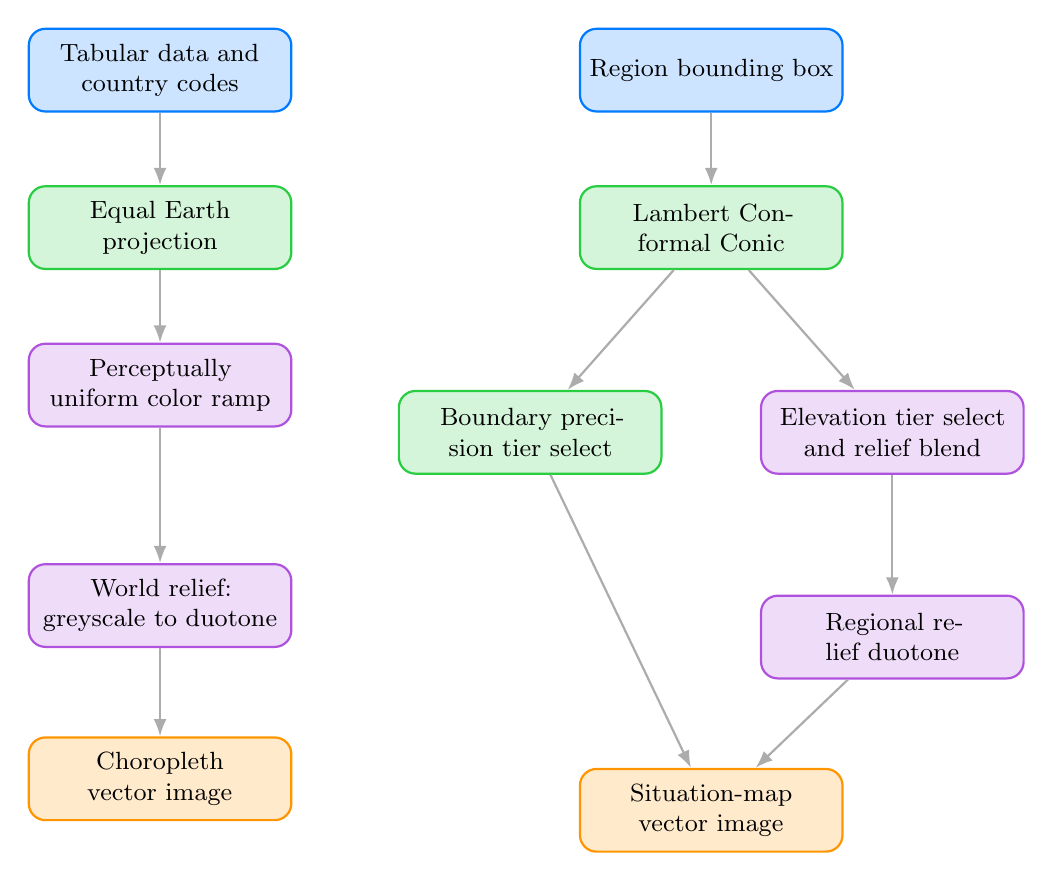
\begin{tikzpicture}
\node[ioNode] (data) at (0,0) {Tabular data and country codes};
\node[ioNode] (bbox) at (7,0) {Region bounding box};
\node[transformNode] (eqearth) at (0,-2) {Equal Earth projection};
\node[transformNode] (lcc) at (7,-2) {Lambert Conformal Conic};
\node[techniqueNode] (ramp) at (0,-4) {Perceptually uniform color ramp};
\node[transformNode] (tier) at (4.7,-4.6) {Boundary precision tier select};
\node[techniqueNode] (elevtier) at (9.3,-4.6) {Elevation tier select and relief blend};
\node[techniqueNode] (worldrelief) at (0,-6.8) {World relief: greyscale to duotone};
\node[techniqueNode] (regionrelief) at (9.3,-7.2) {Regional relief duotone};
\node[outputNode] (choroplethsvg) at (0,-9) {Choropleth vector image};
\node[outputNode] (mapsvg) at (7,-9.4) {Situation-map vector image};

\draw[arr] (data) -- (eqearth);
\draw[arr] (bbox) -- (lcc);
\draw[arr] (eqearth) -- (ramp);
\draw[arr] (lcc) -- (tier);
\draw[arr] (lcc) -- (elevtier);
\draw[arr] (ramp) -- (worldrelief);
\draw[arr] (elevtier) -- (regionrelief);
\draw[arr] (worldrelief) -- (choroplethsvg);
\draw[arr] (tier) -- (mapsvg);
\draw[arr] (regionrelief) -- (mapsvg);
\end{tikzpicture}
\caption{Both generators' pipelines, from input to a finished vector image.}
\end{figure}

\clearpage
\section{World scale: choropleth}

\subsection{Equal Earth projection}

A world choropleth encodes a quantity in each country's fill color, so
the area a projection assigns to a country is not decorative. A
projection that inflates high-latitude land, the classic failure of
Mercator and, less obviously, of a plain equirectangular grid, which
inflates Greenland to roughly fourteen times its true relative size on
this dataset, visually overweights whatever that inflated country's
value happens to be. The fix is an equal-area projection: one where
every region's projected area stays proportional to its true area on
the sphere, by construction.

\texttt{choropleth} uses Equal Earth \autocite{savric-equal-earth}, a
pseudocylindrical equal-area projection published in 2018 as a
deliberately more visually balanced alternative to the older Mollweide
and Robinson projections. Robinson, for reference, is not equal-area at
all; Equal Earth was designed to keep Robinson's pleasant continental
proportions while actually holding the equal-area guarantee Robinson
lacks. It has a closed-form forward projection with published
polynomial constants, so no iteration is required.

Forward projection, for longitude $\lambda$ and latitude $\varphi$ in
radians:

\[
\theta = \arcsin\!\left(\frac{\sqrt{3}}{2}\sin\varphi\right)
\]

\[
x = \frac{\lambda \cos\theta}{\dfrac{\sqrt3}{2}\left(A_1 + 3A_2\theta^2 + \theta^6\left(7A_3 + 9A_4\theta^2\right)\right)}
\]

\[
y = \theta\left(A_1 + A_2\theta^2 + \theta^6\left(A_3 + A_4\theta^2\right)\right)
\]

with the published constants $A_1 = 1.340264$, $A_2 = -0.081106$,
$A_3 = 0.000893$, $A_4 = 0.003796$. This is implemented verbatim in
\texttt{\_equal\_earth\_raw} (\texttt{scripts/make\_choropleth.py:77}). The
projected point cloud's bounding box is fit to the canvas with a single
uniform scale factor, never an independent horizontal or vertical
stretch, since an anisotropic stretch would undo the equal-area property
the whole projection was chosen for.

Equal Earth has no closed-form inverse: $y(\theta)$ is a degree-nine odd
polynomial with no algebraic root formula. The relief layer described
below needs the inverse, to know which real-world longitude and
latitude sits under a given canvas pixel, so
\texttt{\_equal\_earth\_invert\_batch}
(\texttt{scripts/make\_choropleth.py:97}) recovers $\theta$ by
Newton-Raphson iteration on

\[
f(\theta) = \theta\left(A_1 + A_2\theta^2 + \theta^6\left(A_3 + A_4\theta^2\right)\right) - y_{\text{target}} = 0,
\]

started from the small-angle linear approximation $\theta_0 = y / A_1$.
That approximation is exact at $\theta = 0$ and close enough over Equal
Earth's whole valid range, $|\theta| \lesssim 65^\circ$, that twelve
Newton iterations converge to 64-bit floating-point precision. Longitude
then falls out of the forward $x$ formula solved for $\lambda$ at the
now-known $\theta$; latitude falls out of inverting
$\theta = \arcsin\!\left(\tfrac{\sqrt3}{2}\sin\varphi\right)$. Country
outlines themselves never need this inverse: they are drawn forward,
from known vertices, so only the relief raster's per-pixel sampling
uses it.

\subsection{Perceptually uniform color: OKLab and OKLCH}

A choropleth's fill color is the whole message, so the color ramp has
to satisfy a property naive interpolation in the standard three-channel
color encoding (red, green, blue, RGB) does not: equal numeric steps in
the data should read as equal perceived steps in color, and a ramp's
midpoint should not accidentally pass through a muddy, desaturated
grey-brown that reads as ``no data'' rather than ``the middle value.''
Interpolating in the standard color encoding almost every screen and
image file assumes (standard RGB, sRGB) fails both tests. Interpolating
in OKLab and OKLCH fixes both: OKLab is a perceptual color space
published by Björn Ottosson in 2020 \autocite{ottosson-oklab}, and OKLCH
is the same space in cylindrical lightness, chroma, hue form. The fix
costs a heavier per-color conversion chain, which stays cheap here since
ramps are pre-baked into small lookup tables of 256 entries rather than
evaluated per pixel at render time.

The forward chain, in \texttt{scripts/\_geo\_colors.py}:

\begin{enumerate}[leftmargin=1.6em]
\item \textbf{Standard RGB, 8 bits per channel, to linear light}, undoing
  the sRGB transfer function (\texttt{\_srgb\_to\_linear}).
\item \textbf{Linear standard RGB to a space modeled on the eye's three
  cone-cell sensitivity curves} (long, medium, short wavelength, LMS),
  Ottosson's published $3\times3$ matrix:
\[
\begin{pmatrix}l\\m\\s\end{pmatrix} =
\begin{pmatrix}
0.4122214708 & 0.5363325363 & 0.0514459929\\
0.2119034982 & 0.6806995451 & 0.1073969566\\
0.0883024619 & 0.2817188376 & 0.6299787005
\end{pmatrix}
\begin{pmatrix}r\\g\\b\end{pmatrix}_{\text{linear}}
\]
\item \textbf{Signed cube root} of each cone response, sign preserved
  rather than discarded, since saturated or out-of-gamut colors can
  produce a negative cone response.
\item \textbf{Cube-rooted cone space to OKLab} $(L, a, b)$, a second
  published matrix:
\[
\begin{pmatrix}L\\a\\b\end{pmatrix} =
\begin{pmatrix}
0.2104542553 & 0.7936177850 & -0.0040720468\\
1.9779984951 & -2.4285922050 & 0.4505937099\\
0.0259040371 & 0.7827717662 & -0.8086757660
\end{pmatrix}
\begin{pmatrix}l'\\m'\\s'\end{pmatrix}
\]
\item \textbf{OKLab to OKLCH}: $C = \sqrt{a^2+b^2}$, $H = \operatorname{atan2}(b, a)$.
\end{enumerate}

\begin{figure}[htbp]
\centering
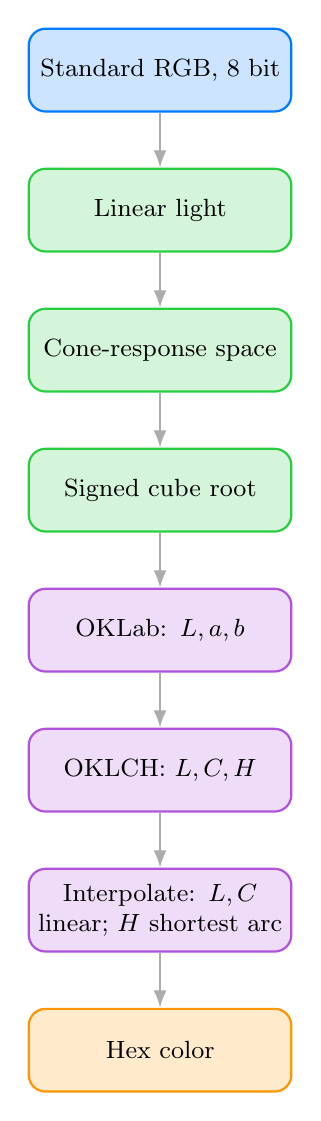
\begin{tikzpicture}[node distance=7mm]
\node[ioNode] (a) {Standard RGB, 8 bit};
\node[transformNode, below=of a] (b) {Linear light};
\node[transformNode, below=of b] (c) {Cone-response space};
\node[transformNode, below=of c] (d) {Signed cube root};
\node[techniqueNode, below=of d] (e) {OKLab: $L,a,b$};
\node[techniqueNode, below=of e] (f) {OKLCH: $L,C,H$};
\node[techniqueNode, below=of f] (g) {Interpolate: $L,C$ linear; $H$ shortest arc};
\node[outputNode, below=of g] (h) {Hex color};
\draw[arr] (a) -- (b);
\draw[arr] (b) -- (c);
\draw[arr] (c) -- (d);
\draw[arr] (d) -- (e);
\draw[arr] (e) -- (f);
\draw[arr] (f) -- (g);
\draw[arr] (g) -- (h);
\end{tikzpicture}
\caption{The forward color chain from a stored hex color to the perceptual space it is interpolated in, and back.}
\end{figure}

Both matrices are inverted exactly (\texttt{\_oklab\_to\_linear},
\texttt{scripts/\_geo\_colors.py:266}) to go back from OKLCH to a hex
color once a ramp stop has been interpolated. Interpolation itself
(\texttt{\_interpolate\_oklch\_hex}, \texttt{scripts/\_geo\_colors.py:424})
treats the three OKLCH channels differently: lightness $L$ and chroma
$C$ interpolate linearly, hue $H$ interpolates along the shorter arc
around the color wheel, so 350 degrees and 10 degrees blend through 0
degrees rather than through 180, and a chroma threshold of $C < 0.01$
guards against interpolating hue through a near-achromatic endpoint.
That guard is not a theoretical nicety. An early version of the
diverging ramp, terracotta fading to a neutral grey, read visibly
mauve or pink at its midpoint, because the two-argument arctangent
function on two near-zero numbers returns a noisy, essentially
arbitrary hue, and interpolating through that noise pulled the midpoint
off course. The fix carries the non-grey endpoint's real hue across the
whole near-achromatic segment instead of trusting the noise.

Two ramp shapes build on this primitive: \texttt{sequential\_ramp\_hex},
pale to navy blue for magnitude, and \texttt{diverging\_ramp\_hex}, which
auto-detects a signed range and picks a below-zero and above-zero color
pair around a neutral midpoint. Every ramp actually shipped is verified,
not merely designed by eye, against three kinds of color-vision
deficiency, meaning conditions where some or all color distinctions are
hard or impossible to perceive (color-vision deficiency, CVD):
protanopia, deuteranopia, and tritanopia, through
\texttt{simulate\_cvd\_hex} (\texttt{scripts/\_geo\_colors.py:627}), which
applies the physiologically derived confusion-line matrices of
\textcite{machado-cvd}. It is also verified against the standard for
measuring whether text stays readable against its background (the Web
Content Accessibility Guidelines, WCAG) contrast-ratio formula, through
\texttt{wcag\_contrast\_ratio} (\texttt{scripts/\_geo\_colors.py:665}), so
a ramp that reads as technically distinct in full color but collapses
to two indistinguishable greys under deuteranopia is caught before it
ships, not discovered later by a color-blind reader.

\begin{figure}[htbp]
\centering
\includegraphics[width=0.92\linewidth]{choropleth-sequential.png}
\caption{Choropleth, sequential ramp: minimum, median, and maximum magnitude on the same dataset.}
\end{figure}

\begin{figure}[htbp]
\centering
\includegraphics[width=0.92\linewidth]{choropleth-diverging.png}
\caption{Choropleth, the same dataset on the auto-detected diverging ramp.}
\end{figure}

\begin{figure}[htbp]
\centering
\includegraphics[width=0.92\linewidth]{cvd-simulation-diverging.png}
\caption{The verification claim above, shown rather than asserted. The shipped diverging ramp, swept end to end, under normal vision and each of the three simulated color-vision deficiencies. The negative, terracotta, and positive, navy, extremes stay distinguishable in every row; only the hue identity of the extremes shifts, never their separability from the neutral midpoint.}
\end{figure}

\subsection{Boundaries: Natural Earth and TopoJSON}

Country outlines come from Natural Earth \autocite{natural-earth}, a
public domain vector and raster atlas published at three fixed scales:
1:110m, 1:50m, and 1:10m, where the number is the map scale the detail
level was drawn for, not a pixel count. \texttt{choropleth} uses the
1:50m tier (\texttt{assets/geo/countries-50m.json}); \texttt{situation\_map}'s
tiering is described in the next section.

The vendored files use TopoJSON, a topology-preserving vector format,
rather than the plain, uncompressed geographic format GeoJSON. TopoJSON
stores shared borders once as reusable arcs rather than once per
adjacent polygon, and quantizes each arc's points to successive integer
deltas rather than raw floating-point coordinates, which is most of why
a TopoJSON file is smaller than the equivalent GeoJSON
\autocite{bostock-topojson}. Decoding an arc
(\texttt{\_decode\_topojson\_object}, \texttt{scripts/make\_situation\_map.py:140})
walks a topology's own scale and translate transform:

\[
x_i = \left(\sum_{k=0}^{i} \delta x_k\right) s_x + t_x, \qquad
y_i = \left(\sum_{k=0}^{i} \delta y_k\right) s_y + t_y
\]

A negative arc index means the decoder should walk that arc reversed,
using a bitwise complement to recover the real index, the encoding
TopoJSON uses so a shared border can be referenced forward by one
polygon and backward by its neighbor without duplicating the
coordinates. Natural Earth's individual country polygons are
occasionally self-touching, invalid in the strict sense defined by the
body that standardizes geographic data formats (the Open Geospatial
Consortium, OGC). Each is repaired with Shapely's \texttt{make\_valid}
before use rather than risking a fragile whole-world union.

\subsection{World relief}

A faint terrain texture sits under the vector layers so the map reads
as a real planet, not a flat color diagram. World scale uses a
different, cheaper technique than the regional path described later: a
pre-rendered greyscale raster (\texttt{assets/geo/relief-lowres.png}, a
1440 by 720 pixel downsample of Natural Earth's public domain ``Gray
Earth'' shaded relief), reprojected by bilinearly sampling it at the
longitude and latitude the Equal Earth inverse recovers for each canvas
pixel (\texttt{sample\_relief}, \texttt{scripts/\_relief.py:194}), then
retinted through a warm and cool duotone lookup table rather than left
as literal grey. That retinting follows Eduard Imhof's ``warm
highlights, cool shadows'' convention \autocite{imhof-relief}: low shade
values, shadowed terrain, map toward a cool blue-slate; high values,
sunlit ridgelines, map toward a warm pale cream; both interpolated
through OKLCH for the same reason the choropleth ramps are. A contrast
stretch runs before the duotone lookup, because the raw raster rarely
spans its own full 0 to 255 range in any single crop (flat ocean sits
at a fixed baseline near 146; even the Himalaya only reaches roughly 90
to 245 in the vendored source), and feeding that narrow band directly
into the duotone lookup table would waste most of its contrast on
values the data never actually reaches.

The regional path's real-elevation technique, described in
Section~\ref{sec:terrain-shading}, does not apply here: a world-scale
crop is too large to run its frequency-domain technique at interactive
cost, and the fine multi-scale texture that technique adds would be
invisible at world zoom regardless.

\begin{figure}[htbp]
\centering
\includegraphics[width=0.92\linewidth]{relief-duotone-comparison.png}
\caption{The same Alps-arc crop of the vendored world raster, plain contrast-stretched greyscale next to the shipped Imhof-style duotone. The duotone version is not merely recolored: it reads with more apparent depth at the same contrast, because the cool-shadow, warm-highlight split gives the eye a second cue, hue, on top of lightness alone.}
\end{figure}

\clearpage
\section{Regional scale: situation\_map}

\subsection{Lambert Conformal Conic, auto-centered}

A regional plate, a single country or a handful of neighboring ones,
needs the opposite property from a world choropleth: not equal area,
but conformality, meaning true local shape and angle, since a viewer
reading a province-level map judges distances and directions locally
rather than by comparing total colored area against a country on the
far side of the globe. \texttt{situation\_map} uses a projection built to
preserve local shape and angle at regional scale, the Lambert Conformal
Conic (LCC) projection, auto-centered on the requested bounding box
(\texttt{build\_projection}, \texttt{scripts/make\_situation\_map.py:371}):

\[
\lambda_0 = \frac{w+e}{2}, \qquad \varphi_0 = \frac{s+n}{2}, \qquad
\varphi_1 = s + \frac{n-s}{6}, \qquad \varphi_2 = n - \frac{n-s}{6}
\]

for a bounding box $[w, s, e, n]$ given as west, south, east, north in
degrees. The two standard parallels $\varphi_1, \varphi_2$, set at the
one-sixth and five-sixths latitudes, follow the classic rule of thumb
for this projection's standard parallels: placing them a sixth of the
way in from each edge, rather than at the edges themselves, keeps the
scale distortion between the parallels and at the region's own edges
comparably small, instead of concentrating all the error at the top and
bottom. The forward and inverse mathematics are delegated to a
dedicated coordinate-transformation library, PROJ \autocite{proj},
through \texttt{pyproj}'s \texttt{Transformer}, not reimplemented. This
projection's own formulas, a true conic projection unlike Equal Earth's
pseudocylindrical family, are well established, and PROJ's
implementation is the reference one, so reimplementing it here would
add risk without adding anything Equal Earth's from-scratch treatment
above did not already cover. That earlier projection needed custom code
specifically because Equal Earth is new enough, published in 2018, that
no equivalent reference implementation existed yet for its inverse.

\begin{figure}[htbp]
\centering
\includegraphics[width=0.92\linewidth]{situation-switzerland.png}
\caption{Situation map, Switzerland.}
\end{figure}

\begin{figure}[htbp]
\centering
\includegraphics[width=0.92\linewidth]{situation-iberia.png}
\caption{Situation map, Iberia.}
\end{figure}

\begin{figure}[htbp]
\centering
\includegraphics[width=0.92\linewidth]{situation-western-europe.png}
\caption{Situation map, Western Europe. Three regions at different scales, the same generator, the same projection family, auto-centered independently for each.}
\end{figure}

\subsection{Boundary tiering}
\label{sec:boundary-tiering-numbers}

Loading the full 1:10m Natural Earth tier for a whole-continent view
spends detail the output cannot show, since individual harbor inlets
are sub-pixel at that zoom, for real cost: a heavier download, a slower
decode, slower geometry operations on more numerous points. Loading
only the coarser 1:50m tier for a single small country, conversely,
visibly under-resolves it: coastlines and small administrative
boundaries read as faceted rather than smooth once a country fills most
of the canvas. \texttt{\_land\_topojson\_for\_bbox}
(\texttt{scripts/make\_situation\_map.py:101}) picks between the two
algorithmically, on the bounding box's own angular span:

\[
\text{tier} =
\begin{cases}
\text{1:10m} & \max(e-w,\, n-s) < 25^\circ \\
\text{1:50m} & \text{otherwise}
\end{cases}
\]

Twenty-five degrees was chosen as roughly the span of a single country
or a small cluster of neighbors, not a subcontinent: Iberia, Spain and
Portugal together, spanning about 13 degrees of longitude, and
Switzerland, spanning under 3 degrees, both resolve to the finer tier;
Western Europe, spanning roughly 41 degrees from Ireland to Poland,
resolves to the coarser one, where the visible gain from finer
coastline detail would not survive the render's own pixel density
regardless.

\subsection{Sub-national admin-1 tiering}
\label{sec:admin1-tiering}

Natural Earth's country boundaries stop at the national frontier: a
situation map zoomed in far enough to fill its canvas with a single
country shows no internal structure at all, an odd gap once the
sub-1:10m detail from Section~\ref{sec:boundary-tiering-numbers} is
already resolving individual coastal inlets. A fourth boundary tier,
one level finer than Natural Earth's admin-0 (country) data, addresses
this: administrative level 1 (admin-1), the first division below the
national level, a state in the United States, a region in France, a
canton in Switzerland. Three national sources were vendored as pilots
for this tier, one per country, each exercising a genuinely different
acquisition path rather than three copies of the same recipe.

\paragraph{TIGER (United States).} The Census Bureau's
Topologically Integrated Geographic Encoding and Referencing (TIGER)
product \autocite{census-tiger} ships as an ordinary Shapefile, public
domain as a U.S.\ government work. Fifty-six state and territory
records (fifty states, the District of Columbia, and five inhabited
territories) were simplified and quantized into a TopoJSON with the
same \texttt{mapshaper} recipe as the admin-0 tiers, fifteen percent
weighted Visvalingam simplification with shape preservation so small
islands survive.

\paragraph{ADMIN EXPRESS (France).} The French national mapping
agency's (Institut Géographique National, IGN) administrative-boundary
product, ADMIN EXPRESS \autocite{ign-adminexpress}, publishes under
France's Licence Ouverte / Etalab 2.0, an attribution license without a
share-alike clause. Eighteen region records (thirteen metropolitan
regions plus five overseas) were fetched from the
\texttt{gregoiredavid/france-geojson} mirror of this dataset, already
in GeoJSON, and vendored through the same \texttt{mapshaper} recipe.

\paragraph{OpenStreetMap (Switzerland).} The third source is
OpenStreetMap itself \autocite{openstreetmap-odbl}, the first dataset
this codebase vendors under the Open Database License (ODbL), and the
one genuinely new acquisition path of the three: OpenStreetMap's
administrative boundaries are not published as ready-made polygon
files but as \emph{relations}, a graph of tagged way segments with
\texttt{outer} and \texttt{inner} roles, queried here through the
Overpass API's \texttt{out geom} mode, which returns each way's own
coordinate list inline rather than a separate node index to resolve.
Switzerland's twenty-six cantons were chosen as the pilot specifically
because several of them, Appenzell Innerrhoden and Appenzell
Ausserrhoden most notably, interleave into mutual enclaves rather than
forming simple single-ring shapes, a real test of the assembly step
rather than a token one. That assembly uses
\texttt{shapely.ops.polygonize}: every \texttt{outer}-role way for a
relation is treated as a graph edge, and \texttt{polygonize} finds the
closed rings the edges form, with \texttt{inner}-role ways run through
the same function and subtracted as holes. No OpenStreetMap PBF
extract, no \texttt{osmium}, no GDAL: one Overpass query and a few
lines of graph assembly.

ODbL's central obligation is attribution on any \emph{produced work},
a rendered map, that draws from it; it does not require the underlying
database to be redistributed, but a vendored extract like
\texttt{assets/geo/ch-cantons.json} \emph{is} itself a derivative
database and therefore carries the same license onward. This codebase
does not leave that obligation for a caller to remember:
\texttt{\_attribution\_layer}
(\texttt{scripts/make\_situation\_map.py}) checks whether the requested
bounding box actually overlaps the vendored Swiss extent, using the
same cheap bounds-overlap pre-check described below, and if so appends
``© OpenStreetMap contributors (ODbL)'' to a small credit line in the
plate's corner automatically, with no configuration required to get
it right and no way to silently omit it while still drawing the
layer.

\subsubsection{The bbox pre-filter pattern}

All three sources share one more piece of shared logic beyond the
\texttt{mapshaper} vendoring recipe: a country boundary
(\texttt{\_US\_STATES\_BOUNDS}, \texttt{\_FR\_REGIONS\_BOUNDS},
\texttt{\_CH\_CANTONS\_BOUNDS}), checked against the requested region's
bounding box before the corresponding TopoJSON file is even read from
disk.

\[
\text{load\_source}(\text{bbox}) =
\begin{cases}
\text{decode and return features} & \text{bbox overlaps source's bounds} \\
[\,] & \text{otherwise}
\end{cases}
\]

This is a bounds overlap, not a true point-in-polygon test, so it is
occasionally a false positive, a region box that touches a source's
bounding rectangle without actually reaching any of its real
geometry, but never a false negative, and the cost of a false positive
is only one avoidable file read, not a wrong border on the plate: the
per-feature intersection check that follows already discards anything
that does not really overlap. The payoff is that
\texttt{\_internal\_borders\_layer} can unconditionally query all
three sources for every situation map, a Himalaya plate included, and
pay nothing beyond three cheap tuple comparisons for the two that do
not apply. The three loaders also share one more piece of code,
\texttt{\_named\_polygons\_from\_topojson}, the arc-decoding and
polygon-repair core factored out once these three sources existed,
rather than duplicated a third and fourth time.

\subsection{Regional relief}

Regional scale replaces the world path's pre-rendered raster with a
technique computed from real elevation data, described in full in the
next section, since it is shared machinery rather than specific to
either generator.

\clearpage
\section{Terrain shading: shared machinery}
\label{sec:terrain-shading}

\texttt{scripts/\_relief.py}'s elevation-based path, distinct from the
world-scale \texttt{sample\_relief} path described above, computes
terrain shading from a global elevation model published in 2010
(Global Multi-resolution Terrain Elevation Data, GMTED2010)
\autocite{danielson-gmted2010}, produced by two United States federal
agencies: the U.S. Geological Survey (USGS) and the National
Geospatial-Intelligence Agency (NGA). The path uses this public domain
model at its finest published grid spacing, 30 arc-seconds, roughly 925
meters per pixel at the equator, where an arc-second is $1/3600$ of a
degree of latitude or longitude. Two shading techniques combine, because
each covers exactly what the other misses.

\textbf{Hillshade} is the familiar technique: a single directional
light source, here a northwest azimuth of $315^\circ$ and an altitude of
$45^\circ$ above the horizon, lights a surface derived from the
elevation grid's own local gradient. Slope and aspect at each cell:

\[
\text{slope} = \arctan\sqrt{\left(\frac{\partial z}{\partial x}\right)^2 + \left(\frac{\partial z}{\partial y}\right)^2}, \qquad
\text{aspect} = \operatorname{atan2}\!\left(\frac{\partial z}{\partial y}, -\frac{\partial z}{\partial x}\right)
\]

with the gradients taken in real meters. Longitude spacing is converted
with a $\cos(\text{latitude})$ correction, since a degree of longitude
shrinks toward the poles while a degree of latitude does not, and
multiplied by a deliberate vertical exaggeration factor, $2\times$ by
default; Section~\ref{sec:exaggeration} explains why. The Lambertian
shading equation itself:

\[
\text{hillshade} = \operatorname{clip}\Big(\sin(\text{alt})\cos(\text{slope}) + \cos(\text{alt})\sin(\text{slope})\cos(\text{az} - \text{aspect}),\; 0,\; 1\Big)
\]

Hillshade alone supplies believable overall lighting and nothing else:
it stays blind to structure much smaller than the light and shadow
transition itself, so fine ridgelines and drainage networks within a
single lit or shadowed face wash out.

\textbf{Texture shading} \autocite{brown-texture-shading} fills exactly
that gap. On certainty: Brown's technique was first circulated at the
2010 conference of a North American professional association for
cartographers (the North American Cartographic Information Society,
NACIS), and formally published at the 2014 Mountain Cartography
Workshop of the worldwide professional body for cartography (the
International Cartographic Association, ICA); both dates appear in the
bibliography entry, since the earlier one is the technique's real
origin but the later one is what has a citable paper. The technique
applies a fractional-order Laplacian in the frequency domain: it
Fourier-transforms the elevation grid using the standard fast algorithm
for computing how a signal decomposes into frequencies (the Fast
Fourier Transform, FFT), multiplies by the frequency magnitude raised
to a fractional power, then inverse-transforms:

\[
T(x,y) = \mathcal{F}^{-1}\Big[\mathcal{F}[z(x,y)] \cdot |\mathbf{f}|^{\alpha}\Big](x,y), \qquad \alpha = 0.5
\]

with $|\mathbf{f}| = \sqrt{f_x^2+f_y^2}$ the spatial-frequency
magnitude and $\alpha$ set within Brown's suggested natural-looking
range of $0.4$ to $0.6$, implemented at $\alpha=0.5$
(\texttt{\_compute\_terrain\_shade}, \texttt{scripts/\_relief.py:575}).
Because this operator scales the whole frequency spectrum by the same
power law rather than isolating one band, it draws out ridge and
drainage structure at every scale simultaneously, which is precisely
what gives texture-shaded relief its engraved, almost etched appearance
compared to a plain lit hillshade. A Hann window is applied to the
elevation crop before the transform, to avoid the ringing a sharp
rectangular crop edge would otherwise inject as spurious high-frequency
content; the crop itself is padded 15 percent beyond the region
actually needed so that window's own edge fade-out lands in a margin
that gets cropped away before reprojection, not inside the visible map.

The two techniques are blended as $0.35 \times \text{hillshade} + 0.65
\times \text{texture}$. Texture-shading output is unbounded and
scale-free, unlike hillshade's physical $[0,1]$ range, so it is
renormalized around its own standard deviation before blending. That
specific ratio, and the choice to run texture shading at all rather
than ship hillshade alone, was not settled by theory: it was calibrated
by direct visual comparison against editorial, New York Times-style
relief cartography, the print-map house style this project takes its
visual cues from, until the output matched, following the Ralph
Eyeball Loop described in Section~\ref{sec:validation}. The resulting
shade grid is retinted through the same Imhof-style OKLCH duotone
lookup table the world-scale path uses (\texttt{\_duotone\_lut},
\texttt{scripts/\_relief.py:133}), so both generators share one visual
language for relief even though they compute it two different ways.

\begin{figure}[htbp]
\centering
\includegraphics[width=0.92\linewidth]{situation-himalaya.png}
\caption{Regional relief on genuinely varied terrain, the Himalaya, where hillshade alone would show only the overall light and dark massif, while texture shading resolves individual ridgelines within it.}
\end{figure}

The two techniques run independently on the same elevation crop and
converge only at the blend step.

\begin{figure}[htbp]
\centering
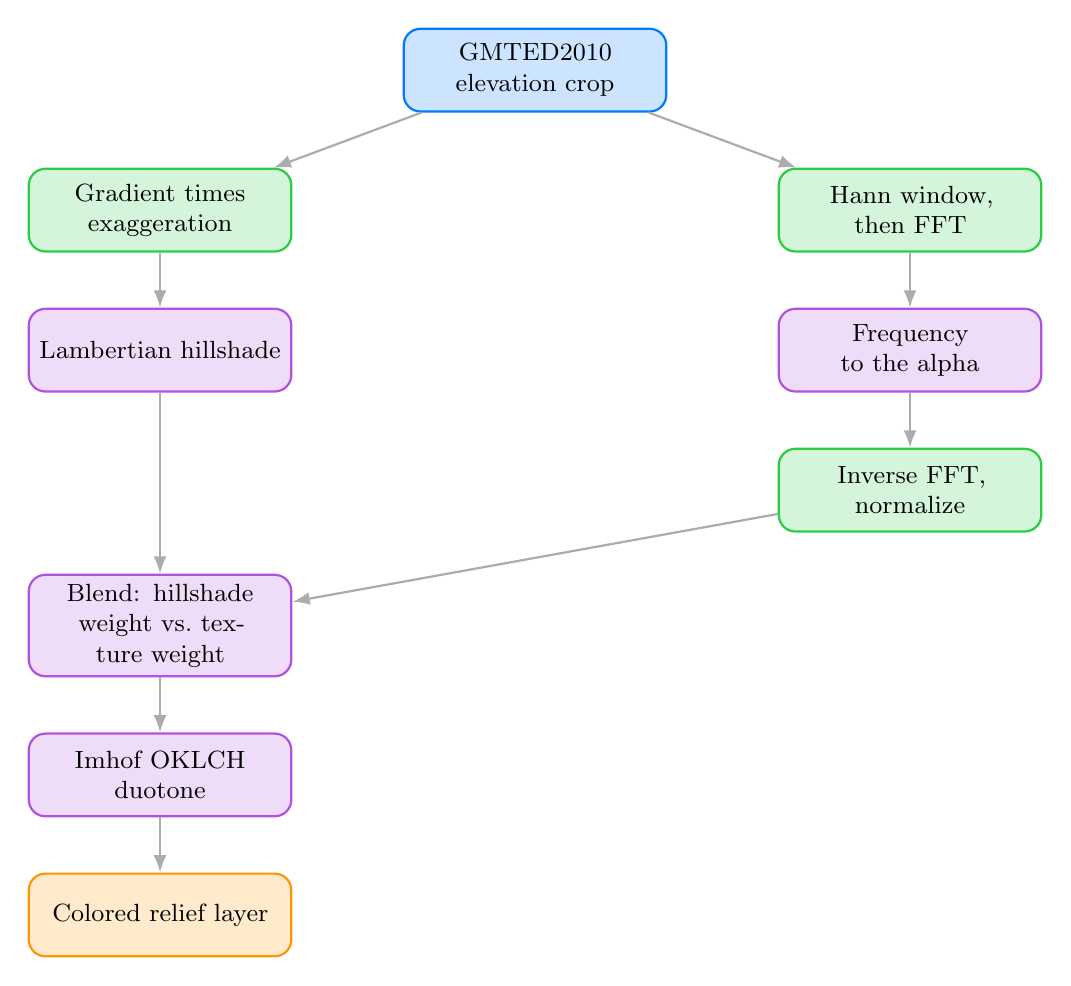
\begin{tikzpicture}[node distance=7mm and 12mm]
\node[ioNode] (a) {GMTED2010 elevation crop};
\node[transformNode, below left=of a, xshift=-0.2cm] (b) {Gradient times exaggeration};
\node[transformNode, below right=of a, xshift=0.2cm] (d) {Hann window, then FFT};
\node[techniqueNode, below=of b] (c) {Lambertian hillshade};
\node[techniqueNode, below=of d] (e) {Frequency to the alpha};
\node[transformNode, below=of e] (f) {Inverse FFT, normalize};
\node[techniqueNode, below=of c, yshift=-1.6cm] (g) {Blend: hillshade weight vs.\ texture weight};
\node[techniqueNode, below=of g] (h) {Imhof OKLCH duotone};
\node[outputNode, below=of h] (i) {Colored relief layer};
\draw[arr] (a) -- (b);
\draw[arr] (a) -- (d);
\draw[arr] (b) -- (c);
\draw[arr] (d) -- (e);
\draw[arr] (e) -- (f);
\draw[arr] (c) -- (g);
\draw[arr] (f) -- (g);
\draw[arr] (g) -- (h);
\draw[arr] (h) -- (i);
\end{tikzpicture}
\caption{Terrain shading's two independent paths, hillshade and texture shading, converging at the blend step.}
\end{figure}

\clearpage
\subsection{Relief exaggeration strategies}
\label{sec:exaggeration}

A perfectly literal, physically accurate render of GMTED2010's real
elevation values would look almost flat. Even the Himalaya, the most
dramatic terrain this dataset has, spans roughly 8800 meters of relief
across hundreds of kilometers: a slope so gentle in true proportion
that a photorealistic light simulation of it reads as a faint grey
haze, not a mountain range. Every relief cartographer's toolkit
therefore includes deliberate departures from physical literalness,
chosen to make the terrain legible rather than to simulate a camera.
\texttt{\_compute\_terrain\_shade} (\texttt{scripts/\_relief.py:576})
exposes three such departures as named parameters,
\texttt{vertical\_exaggeration}, \texttt{texture\_alpha}, and
\texttt{hillshade\_weight}, each with a shipped default
(\texttt{DEFAULT\_VERTICAL\_EXAGGERATION = 2.0},
\texttt{DEFAULT\_TEXTURE\_ALPHA = 0.5},
\texttt{DEFAULT\_HILLSHADE\_WEIGHT = 0.35}, \texttt{scripts/\_relief.py:575}),
so the same production code path used for every real render also
produces the comparison figures below, rather than a separate script
reimplementing the algorithm at different settings.

\textbf{Vertical exaggeration} is the oldest and most literal strategy:
multiply the elevation gradient by a constant before it becomes a
hillshade slope angle, so the same light source casts a harder, more
legible shadow than the true slope would produce. It is a
spatial-domain exaggeration, applied uniformly to the whole gradient
regardless of the terrain feature's own size.

\begin{figure}[htbp]
\centering
\includegraphics[width=0.92\linewidth]{relief-exaggeration-vertical.png}
\caption{The same Everest-massif crop, hillshade only, with texture-shading weight set to zero to isolate this one variable, at true scale versus the shipped $2\times$ default. Ridgelines barely readable at true scale separate cleanly at the shipped setting, without yet introducing any of texture shading's own contribution.}
\end{figure}

\textbf{Texture shading's fractional order} $\alpha$, introduced in the
formula above, is a different kind of exaggeration: not spatial but
spectral. Instead of stretching every gradient by the same factor
regardless of the feature size it belongs to, it boosts every spatial
frequency of the elevation field by the same power law at once, so a
tiny side valley's drainage pattern is exaggerated by the same
proportional amount as the main massif's ridgeline, rather than being
swamped by it. This is what lets texture shading resolve structure
within a single hillshade-lit face that vertical exaggeration alone
cannot touch, since a spatial gradient stretch cannot separate a pixel
on a ridge from a pixel on a valley wall once both already fall on the
same broad lit slope.

\textbf{The blend weight} between the two is the third strategy, and
the one that decides whether the final image reads as a lit photograph
or an engraved diagram. Hillshade alone is the physically motivated,
photograph-like extreme; texture shading alone is the abstract,
frequency-only extreme, which on its own looks more like a printed
circuit board than a mountain, since it discards the overall light and
dark massif shape that only hillshade's directional lighting supplies.
The shipped $0.35/0.65$ split sits deliberately close to the texture
end without discarding hillshade's contribution entirely.

\begin{figure}[htbp]
\centering
\includegraphics[width=0.92\linewidth]{relief-exaggeration-blend.png}
\caption{The same crop decomposed into its two ingredients and their shipped blend. Hillshade alone supplies a believable overall lit surface but reads soft; texture shading alone supplies extraordinary fine detail but reads abstract, closer to an X-ray than a mountain; the shipped blend keeps hillshade's photographic legibility while letting texture shading's drainage-network detail read through it, the combination this project's whole relief system was built to reach.}
\end{figure}

The figures above are regenerable in one command against the real
vendored elevation data, whenever any of the three defaults changes:

\begin{verbatim}
python scripts/build_relief_exaggeration_figures.py
\end{verbatim}

The world-scale path described earlier has no elevation grid to apply a
vertical or spectral exaggeration to, since it works from a single
pre-shaded raster rather than raw elevation. Its analogous exaggeration
strategy is purely tonal: the contrast stretch described earlier
(\texttt{\_SHADE\_STRETCH\_LOW} and \texttt{\_SHADE\_STRETCH\_HIGH},
\texttt{scripts/\_relief.py:113}) remaps whatever narrow grey-value
range a given crop actually occupies back out to the duotone lookup
table's full contrast range: the same underlying goal, making faint
real terrain read clearly, reached through the one lever a
pre-rendered raster leaves available.

\subsection{Elevation pyramid and algorithmic tier selection}

The finest GMTED2010 tier is a 902 million pixel grid, about 237
megabytes as a 16-bit lossless raster image (Portable Network Graphics,
PNG) file. Loading it for every render, including a whole-continent
view where individual valleys are sub-pixel anyway, spends real time and
memory on detail the output cannot show. \texttt{select\_elevation\_tier}
(\texttt{scripts/\_relief.py:388}) picks the coarsest of six mipmap-style
pyramid tiers, from 30 arc-seconds down to 16 arc-minutes, each an
exact $2\times2$ block average of the tier above it so the levels stay
mutually consistent rather than being independently resampled from the
source, that still comfortably resolves the requested render:

\[
\Delta_{\text{out}} = \min\!\left(\frac{e-w}{\,w_{\text{px}}\,},\ \frac{n-s}{\,h_{\text{px}}\,}\right), \qquad
\Delta_{\text{budget}} = \frac{\Delta_{\text{out}}}{k}
\]

where $\Delta_{\text{out}}$ is the render's own angular resolution in
degrees per output pixel, taking the more demanding of the two axes,
$k$ is an oversample factor with a default of $2.0$, and the chosen
tier is the coarsest one whose own pixel spacing in degrees is still
at most $\Delta_{\text{budget}}$. Oversampling beyond a literal one-to-one
pixel match matters specifically because texture shading draws out
fractal structure below the output's own pixel size, which then
anti-aliases into the final bilinearly resampled image; a tier that
only just matches output resolution measurably softens the result,
which is exactly what an earlier, single-fixed-tier version of this
system showed on inspection. The oversample factor of $2.0$ was
calibrated against the same three regions used throughout this
document: at that setting, Iberia and Switzerland's actual bounding
boxes still resolve to the finest 30 arc-second tier, matching what
visual comparison against the editorial reference cartography above
showed was needed, while Western Europe's much larger bounding box
drops to 1 arc-minute with no visible loss at that render scale.

\clearpage
\section{Data provenance and licensing}

\begin{table}[htbp]
\centering
\small
\begin{tabular}{p{3.6cm}p{3.4cm}p{3.4cm}p{2.6cm}}
\toprule
Dataset & Source & License & Used by \\
\midrule
Country and coastline boundaries (110m, 50m, 10m) & Natural Earth \autocite{natural-earth} & Public domain & Both generators \\
World relief raster & Natural Earth ``Gray Earth'' & Public domain & \texttt{choropleth} \\
Global elevation grid (GMTED2010, 30 arc-sec) & USGS/NGA \autocite{danielson-gmted2010} & Public domain (U.S.\ government work) & \texttt{situation\_map} \\
Rivers and lake centerlines (1:50m) & Natural Earth & Public domain & \texttt{situation\_map} \\
US state boundaries (TIGER/Line) & U.S.\ Census Bureau \autocite{census-tiger} & Public domain & \texttt{situation\_map} \\
France region boundaries (ADMIN EXPRESS) & IGN, via \texttt{france-geojson} \autocite{ign-adminexpress} & Licence Ouverte / Etalab 2.0 & \texttt{situation\_map} \\
Switzerland canton boundaries & OpenStreetMap \autocite{openstreetmap-odbl} & ODbL 1.0 (attribution required) & \texttt{situation\_map} \\
\bottomrule
\end{tabular}
\caption{Every dataset this codebase vendors, its license, and which generator uses it.}
\end{table}

Every dataset in this table above the three admin-1 boundary rows is
usable with no attribution obligation, though Natural Earth's own
suggested short citation, ``Made with Natural Earth,'' is honored here
regardless, since it costs nothing and this document already cites
everything else. The Switzerland canton row is the one exception, and
the first dataset this codebase vendors under a share-alike or
attribution-required license: OpenStreetMap's Open Database License
requires attribution on any produced work that draws from it, which
\texttt{\_attribution\_layer} adds automatically rather than leaving
to a caller to remember, described in full in
Section~\ref{sec:admin1-tiering}.

\section{Storage: the vendored-raster pyramid and Git LFS}

Every raster asset this document describes, \texttt{relief-lowres.png}
and the six-tier \texttt{elevation-*.png} pyramid, is vendored in the
repository rather than fetched at render time, so a render stays
reproducible offline and does not depend on a third-party host staying
up. Because these files range from a few hundred kilobytes to 237
megabytes, they are tracked with a Git extension that stores large
binary files outside the main repository history (Large File Storage,
LFS) rather than committed as ordinary blobs, through a single
\texttt{assets/geo/*.png filter=lfs diff=lfs merge=lfs -text} rule in
\texttt{.gitattributes}, so the main repository history stays small and
a clone only pulls the actual raster bytes when they are checked out or
explicitly fetched. The same pattern, vendor once, keep a lightweight
pyramid of derived tiers, pick a tier algorithmically at render time
rather than by a hardcoded choice, extends to boundary data too, the
admin-0 country tiers already, and the admin-1 sources described in
Section~\ref{sec:admin1-tiering} now as well; see the roadmap in
Section~\ref{sec:roadmap} for how far that extension still has to go.

\section{Validation methodology}
\label{sec:validation}

Every relief and color change described above went through what this
project calls the Ralph Eyeball Loop: render, inspect the actual raster
output rather than only check that the code ran without raising an
error, critique against a concrete target such as a reference image or
a specific defect like visible blockiness or a muddy ramp midpoint,
edit the source, and render again, never editing the output image
directly. Two smaller mechanical checks back this at the code level:
every public function in \texttt{scripts/\_relief.py} and
\texttt{scripts/\_geo\_colors.py} carries a doctest exercising its
documented contract, run with \texttt{python -m doctest scripts/\_relief.py}
and the equivalent for \texttt{\_geo\_colors.py}, and the full test suite,
run with \texttt{pytest -q}, additionally covers the command-line,
web-service, and model-context-protocol surfaces end to end. Neither
check catches a visually wrong result on its own: a hillshade that runs
without error and returns the right array shape can still look flat.
The Ralph Eyeball Loop is what catches that category of defect, and the
doctest and test-suite layer is what keeps a later refactor, the
tier-selection rewrite described above, for one, from silently breaking
a contract the eyeball pass already validated.

\section{Roadmap}
\label{sec:roadmap}

The admin-1 boundary tier described in
Section~\ref{sec:admin1-tiering}, TIGER for the United States, ADMIN
EXPRESS for France, OpenStreetMap for Switzerland, closes what had
been this document's longest-standing open item: a fourth boundary
tier above Natural Earth's 1:10m, for renders zoomed in far enough to
need sub-1:10m-scale accuracy, plus the licensing groundwork ODbL
required, now in place and exercised by a real dataset rather than
only discussed. What remains is the coverage this pilot deliberately
left out, listed here rather than left silently implied, on the
principle that a document like this one should mark what is done and
what is not with the same explicitness.

\begin{itemize}[leftmargin=1.4em]
\item \textbf{Coverage beyond the three pilot countries}: admin-1
  boundaries exist today only for the United States, France, and
  Switzerland, one source per source type rather than a general
  worldwide layer. The OpenStreetMap/Overpass path in particular
  generalizes directly, the same \texttt{outer}/\texttt{inner}
  \texttt{polygonize} assembly works for any country's
  \texttt{admin\_level=4} relations, a different admin level entirely
  in countries where 4 is not the state-equivalent tier, so the next
  country is a query and a vendoring pass, not new code.
\item \textbf{A finer admin-2 tier} (US counties, French departments,
  Swiss districts) below the admin-1 layer just added, for renders
  zoomed in past a single state, region, or canton, the same
  relationship admin-1 now has to Natural Earth's admin-0.
\item \textbf{Applying this document's storage pattern}, vendor once,
  keep a multi-resolution pyramid, pick a tier algorithmically at
  render time, more fully to boundary data: the bbox pre-filter
  pattern in Section~\ref{sec:admin1-tiering} already picks
  algorithmically \emph{which source} applies, US, France, or
  Switzerland, but each individual source is still a single
  resolution rather than its own pyramid the way
  \texttt{select\_elevation\_tier} gives elevation six tiers.
\end{itemize}

\clearpage
\printbibliography

\end{document}
